%
% ichep2018_proceedings.tex
% Matt Solt & Omar Moreno, SLAC National Accelerator Laboratory
%

\documentclass[twocolumn, showpacs, preprintnumbers,prd, superscriptaddress]{revtex4-1}
\pdfoutput=1

\usepackage{color}
\usepackage{cancel}
\usepackage{epstopdf}
\usepackage{epsfig}
\usepackage{booktabs}
 \usepackage{array,multirow}

%%%%%%%%%%%%%%%%
%   Packages   %
%%%%%%%%%%%%%%%%

% Package from AMS that facilitates formula typography
\usepackage{amsmath, amssymb, mathrsfs}

% LaTex graphics package
\usepackage{graphicx}

% Package used to manipulate the document header and footer
\usepackage{fancyhdr}

% Align table columns on decimal point
\usepackage{dcolumn}

% Use bold math
\usepackage{bm}

% Set the encoding of the document
\usepackage[utf8]{inputenc}

% Package used to add hyperlinks to references within a document
\usepackage{hyperref}

% Package used to add colors to text
\usepackage{xcolor}

% 
\usepackage{footnote}

%\setlength{\parskip}{.1cm plus0mm minus0mm}

\newcommand{\mevcc}{MeV/c$^2$}
\newcommand{\gevcc}{GeV/c$^2$}
\newcommand{\pos}{e^{+}}
\newcommand{\ele}{e^{-}}
\newcommand{\epem}{\pos\ele}
\newcommand{\emem}{\ele\ele}
\newcommand{\re}[1]{\textcolor{red}{[RE: #1]}}
\newcommand{\aprime}{A^\prime}

\begin{document}

    %\preprint{JLAB-PHY-XX-XXXX/SLAC-PUB-XXXXX}

	\title{Search for a Dark Photon in Electro-Produced $\epem$ Pairs 
    	   with the Heavy Photon Search Experiment at JLab}
    
    %
% 2018 ICHEP Proceedings Author List
%
%

\newcommand*{\SLAC}{SLAC National Accelerator Laboratory, Stanford University, Stanford, CA 94309, USA}
\newcommand*{\SLACindex}{49}
\newcommand*{\UCSC}{Santa Cruz Institute for Particle Physics, University of California, Santa Cruz, CA 95064, USA}
\newcommand*{\UCSCindex}{50}

\author{M.~Solt}\email[Corresponding author, email:]{mrsolt@slac.stanford.edu}\affiliation\SLAC
\author{O.~Moreno}\affiliation\SLAC\affiliation\UCSC


    %\hspace{10pt}   

    %\normalsize 
    %    Matt Solt$^1$\footnote{
    %        \noindent Corresponding author. E-mail: mrsolt@slac.stanford.edu
    %    },
    %    Omar Moreno$^1$

    %\hspace{10pt}

    %$^1$\emph{SLAC National Accelerator Laboratory, Menlo Park, CA 94205} \\ 
    
    \date{\today}
    
    \begin{abstract}
        
        The Heavy Photon Search experiment took its first data in a 2015
        engineering run at the Thomas Jefferson National Accelerator Facility,
        searching for a prompt, electro-produced dark photon with a mass 
        between 19 and 81~\mevcc. A search for a resonance in the $\epem$
        invariant mass distribution, using 1.7 days (1170 nb$^{-1}$) of data, 
        showed no evidence of dark photon decays above the large QED background,
        confirming earlier searches and demonstrating the full functionality of
        the experiment. Upper limits on the square of the coupling of the dark
        photon to the Standard Model photon are set at the level of 
        6$\times$10$^{-6}$. Future runs with higher luminosity will explore new 
        territory. 

	\end{abstract}
	
	\pacs{14.70.Pw, 25.30.Rw}
    
    \maketitle
    
    \section{Introduction}
        
        The search for low-mass hidden sectors weakly coupled to the Standard 
        Model (SM) has received increased attention over the last
        decade~\cite{Hewett:2012ns,Essig:2013lka,Alexzzander:2016aln,
        Battaglieri:2017aum,Jaeckel:2010ni}.   Hidden sectors are motivated by
        the existence of dark matter, appear in myriad extensions of the SM, 
        and have been invoked to explain a wide variety of experimental anomalies.   

        A prototypical hidden sector consists of a spontaneously broken 
        ``hidden'' $U(1)'$ gauge symmetry, whose mediator is the 
        ``heavy photon'' or ``dark photon'', $\aprime$.  The heavy photon
        interacts with SM particles through kinetic mixing with the $U(1)_Y$ 
        (hypercharge) gauge boson~\cite{Holdom:1985ag,Galison:1983pa}, 
        resulting in the effective lagrangian density
        \begin{equation} \label{kmix} 
            {\cal L} \supset -\frac{\epsilon}{2\cos\theta_W} F'_{\mu\nu} F^{\mu\nu}_Y\,. 
        \end{equation}
        Here $\epsilon$ is a dimensionless coupling parameter, $\theta_W$ is the 
        Weinberg mixing angle, 
        $F'_{\mu\nu}=\partial_{\mu}\aprime_{\nu}-\partial_{\nu}\aprime_{\mu}$ 
        is the $U(1)'$ field strength, and similarly $F^{\mu\nu}_Y$ denotes the
        SM hypercharge $U(1)_Y$ field strength. This mixing generates an 
        interaction between the $\aprime$ and the SM photon at low energies,  
        allowing dark photons to be produced in charged particle interactions
        and, if sufficiently massive, to decay into pairs of charged particles 
        like $\epem$ or hidden-sector states.  The value of $\epsilon$ is 
        undetermined, but a value of $\epsilon^2 \sim 10^{-8}-10^{-4}$ is 
        natural if generated by quantum effects of heavier particles charged
        under $U(1)'$ and $U(1)_Y$.  If the SM forces unify in a Grand Unified 
        Theory, then $\epsilon^2 \sim 10^{-12}-10^{-6}$ is 
        natural~\cite{ArkaniHamed:2008qp,Baumgart:2009tn,Essig:2009nc}.  
        The mass of the $A'$, $m_{A'}$, is also undetermined, but the MeV-to-GeV
        mass scale has received much attention over the last decade as a 
        possible explanation for various anomalies related to dark matter
        interacting through the $A'$~\cite{ArkaniHamed:2008qn,Pospelov:2008jd,
        Finkbeiner:2007kk,Fayet:2004bw,Kaplinghat:2015aga} and for the 
        discrepancy between the observed and SM value of the muon anomalous 
        magnetic moment~\cite{Pospelov:2008zw,Bennett:2006fi,Davier:2010nc}.  
        Moreover, this mass range appears naturally in a few specific
        models~\cite{ArkaniHamed:2008qp,Cheung:2009fk,Baumgart:2009tn,
        Morrissey:2009ur,Essig:2009nc}. 

        The Heavy Photon Search (HPS) is an experiment utilizing the CEBAF
        accelerator at the Thomas Jefferson National Accelerator Facility (JLab)
        in Newport News, Virginia, USA. The experiment can explore a wide range
        of masses ($m_{\aprime}\sim 20-500$~\mevcc) and couplings 
        ($\epsilon^2 \sim 10^{-6} - 10^{-10}$), using both resonance search and
        separated vertex strategies. In this paper, results of a 
        resonance search from a Spring 2015 engineering run  
        using a 50~nA, 1.056~GeV electron beam impinging on a
        thin (0.125\%$X_{0}$) tungsten target are reported.  Electron interactions 
        with the 
        target nuclei could produce an $A'$ particle, which could subsequently 
        decay to an $\epem$ 
        pair~\cite{Bjorken:2009mm,Reece:2009un,Freytsis:2009bh}. A spectrometer,
        triggered by an electromagnetic calorimeter, measures the momenta and
        trajectories of this pair, allowing for the reconstruction of its
        invariant mass and decay position. The $\aprime$ would appear as a 
        narrow resonance, with a width set by the mass resolution, on top of a 
        smooth and wide distribution of background events from ordinary
        quantum electrodynamic (QED) processes.

        The cross section for  $\aprime$ production and subsequent decay to $\epem$      
        (``radiative $\aprime$ production'') scales with $\epsilon^2$ and is 
        directly proportional to the cross section for $\epem$ pair production
        from virtual photon bremsstrahlung 
        (``radiative trident production'')~\cite{Bjorken:2009mm}, so their
        yields are proportional. We assume the
        $\aprime$ only decays to $\epem$, as expected below the di-muon threshold
        if there are no invisible $\aprime$ decays.
        The measured $\epem$ yield, $dN/dm_{\aprime}$, is accounted for by
        the sum of trident and wide-angle bremsstrahlung (WAB) processes. Both
        radiative and Bethe Heitler diagrams contribute to trident production.
        WABs contribute if the photon converts and the resulting positron is detected
        along with the electron which has radiated.
        After accounting for the converted WABs, the trident yield is known.
        The fraction
        of all tridents which are radiative can be calculated, so the radiative trident
        yield is also determined, fixing the sensitivity of the search. 
        The experimental mass resolution impacts the experimental reach and is a
        critical input to the fits of the mass spectrum; it is calibrated by 
        measuring the invariant mass of M\o ller pairs, which have a unique 
        invariant mass for any given incident electron energy.

        The outline of the rest of the paper is as follows. 
        In Sec.~\ref{sec:detector}, we describe the experimental setup and the
        detector. Sec.~\ref{sec:selection} discusses the selection of the 
        events to maximize the $A'$ signal over the QED background.  
        Sec.~\ref{sec:resonance} describes the analysis of the resonance search,
        while Sec.~\ref{sec:results} presents the results.  Our conclusions are 
        presented in Sec.~\ref{sec:conclusions}. 
   
    \section{Detector Overview}\label{sec:detector}	
        
        The kinematics of $\aprime$ electro-production result in very 
        forward-produced heavy photons, which carry most of the beam energy and decay to
        highly-boosted $\epem$ pairs. To accept these decays, the HPS detector is 
        designed as a compact forward magnetic spectrometer, consisting of a silicon
        vertex tracker (SVT) placed in a vertical dipole magnetic field for momentum
        measurement and vertexing, and a PbWO$_4$ crystal electromagnetic calorimeter
       (ECal) for event timing and triggering. The SVT consists of six layers of
        detectors located in vacuum between 10 and 90 cm from the target, and
        arranged just above and below the ``dead zone'', a horizontal fan of intense
        flux from beam particles which have scattered or radiated in the target.
        Each
        layer consists of two silicon microstrip sensors with a small (50 or 100
        mrad) stereo angle for three dimensional position 
        determination~\cite{Adrian:2018}. The ECal  has 442 crystals and is situated downstream of the 
        tracker~\cite{Balossino:2016nly}. The ECal is split above and below the
        vacuum chamber which transports the beam towards the dump.
        
        HPS searches for a small signal above the much larger QED trident background, 
        so it must accumulate high statistics. This was
        accomplished using CEBAF's nearly continuous beam, 
        SVT and ECal readout with precision timing, and a high rate data acquisition
        system. The CEBAF accelerator provided a very stable beam with negligible
        halo, focused to a $\sim$100 $\mu$m spot at the 
        target~\cite{Baltzell:2016eee}. The SVT was read out using the APV25 ASIC operating at 41.333 MHz~\cite{French:2001xb} and triggered data from each sensor was sent to the SLAC ATCA-RCE readout system~\cite{Herbst:2016prn}. The ECal was read out with a 250 MHz 
        JLab FADC~\cite{Dong}. A custom trigger used the ECal information to
        select events consistent with coming from a high-energy $\epem$ pair.
        The data acquisition system could record events at rates up to 25 kHz with less than 15\% deadtime.
        
        The  analyzing magnet provided a field of 0.25 Tesla. The resulting
        SVT momentum resolution is $\delta p/p = 7$\% for beam energy electrons
        and is approximately constant for all momenta of 
        interest~\cite{Adrian:2018}. The ECal has an energy resolution 
        $\delta E/E = 5.7$\% at 0.5 GeV with significant energy and position
        dependence~\cite{Balossino:2016nly}. Using 
        information from the ECal and the SVT, we select $\epem$ pairs and
        reconstruct their invariant mass and vertex positions. This gives the
        experiment access to two regions of parameter space, comparatively
        large couplings using a traditional resonance search strategy, and very small 
        couplings using the distance from the target to the decay vertex to
        eliminate almost all of the prompt 
        trident background.      
        
        The HPS detector was installed and commissioned within the Hall B
        alcove at JLab early in the spring of 2015 and subsequently took its
        first data.  In total, 1170 nb$^{-1}$ of data was collected 
        (corresponding to 7.25 mC of integrated charge), equivalent to 
        1.7 days of continuous running. 

\section{Resonance Search Event Selection}\label{sec:bhselection}
    
    	Searching for a heavy photon resonance requires accurate
        reconstruction of the $\epem$ invariant mass spectrum; 
        rejection of background events due to converted WAB events, non-radiative
        tridents from the Bethe-Heitler process, 
        and occasional accidental $\epem$ pairs; and efficient selection of $\aprime$ candidates.     
        Selecting $\aprime$ candidates is equivalent to selecting
        radiative tridents since they have identical kinematics for a
        given mass. In order to perform a blind search, the event selection  was 
        optimized using $\sim$10\% of the 2015 engineering run dataset.
        
        Heavy photon candidates are created from pairs of electron and positron
        tracks, one in each half of the SVT, each of which point to an energy  
        cluster in the ECal.  Each track must pass loose quality requirements
        and have a reconstructed momentum less than 75\% of the beam energy
        (0.788 \gevcc) to reject scattered beam electrons.  The background from 
        accidental pairs was reduced to less than 1\% by requiring the time between 
        the ECal clusters be less than 2 ns and the time between a track and the
        corresponding cluster be less than 5.8 ns.
        
        Heavy photons decay to highly boosted $\epem$ pairs, while the 
        recoiling electron is soft, scatters to large angles, and is usually
        undetected. Radiative tridents, having identical kinematics, comprise
        an irreducible background. The Bethe-Heitler diagram also contributes
        to trident production, and in fact dominates over the radiative process
        at all pair momenta. This background is minimized by requiring the
        momentum sum of the $\epem$ pair to be greater than 80\% of the beam
        energy (0.84 \gevcc), where the radiative tridents are peaked.
        
        The other significant source of background arises from converted WAB 
        events in which the bremsstrahlung photon is emitted at a large angle
        ($>15$ mrad), converts in the target, first or second layer of the SVT, and 
        gives rise to a detected positron in the opposite half of the detector 
        from the recoiling incoming electron. Although the fraction of such 
         WAB events that convert with this topology  is extremely low, 
        it is offset by the fact that 
        the bremsstrahlung rate is huge compared to the trident rate. This 
        results in converted WAB events making up roughly 30\% of our sample.  
        
        The converted WAB background was substantially reduced by applying additional 
        selection criteria. Since the conversion usually happens in the
        first layers of the silicon detector, requiring both tracks to have 
        hits in the first two layers of the SVT removes most of the converted WABs. 
        %This removes about XXXOM\% of the converted WAB events.  
        Requiring the transverse momentum asymmetry between the
        electron and positron be 
        $\frac{p_t(\ele)-p_t(\pos)}{p_t(\ele)+p_t(\pos)}<0.47$ and the 
        transverse distance of closest approach to the beam spot of the 
        positron track to be less 
        than 1.1 mm removes many of the remaining conversions. With all these cuts,
        contamination from converted WABs is reduced to 12\%.  
	
	    The composition of our event sample was checked by comparing the rates
        and distributions of several key variables (e.g total pair energy, 
        electron energy, positron energy, and invariant mass) between data and
        Monte Carlo (which included tridents, converted WABs, and accidental 
        background). We find that the data and MC are in reasonable agreement. 

    \section{Resonance Search}\label{sec:resonance}
       
        A heavy photon is expected to appear as a Gaussian-shaped resonance above the
        $\epem$ invariant mass spectrum, centered on the $\aprime$ mass and
        with a width, $\sigma_{m_{\aprime}}$, which characterizes the 
        experimental mass resolution.  M\o ller scattering events 
        ($\emem \rightarrow \emem$) are used to calibrate the $\aprime$ mass 
        scale and resolution.  Figure~\ref{fig:mass_resolution} shows the 
        measured M\o ller invariant mass, after a series of quality and 
        selection cuts.  For incident electrons of energy 1.056 GeV, we observe
        a M\o ller mass peak of 33.915 $\pm$ 0.043 MeV, within 1\% agreement of
        the expected mass of 34.1 MeV.  The M\o ller mass resolution predicted
        by Monte Carlo is 1.30 $\pm$ 0.02 MeV, in contrast with the observed 
        value of 1.61 $\pm$ 0.04 MeV.  We ascribe the difference to the fact 
        that our measured momentum resolution for beam energy electrons (7.03\%) 
        is significantly worse than predicted by Monte Carlo (5.9\%). Since
        the mass resolution scales directly with the momentum resolution, it 
        is underestimated in Monte Carlo by 19\%.  Consequently, we scale up
        the simulated $\aprime$ mass resolution by a factor of 1.19.
        The resulting parameterization of the mass resolution is an input to the 
        resonance search.
        
        \begin{figure}[th]
            \centering
            \includegraphics[width=.9\linewidth]{moller_invariant_mass_fit.pdf}
            \caption{
                The M\o ller mass peak used to measure the mass resolution.
                The peak was fit with a Crystal Ball function plus a Gaussian
                for the tail at high mass. The $\sigma$ of the Crystal Ball 
                function was taken as the mass resolution. The overall fit is 
                in red; the core Crystal Ball in dashed blue.}
            \label{fig:mass_resolution}
        \end{figure}

        Since the mass of a putative $\aprime$ is unknown a priori, the entire 
        $\epem$ invariant mass spectrum is scanned for any significant peaks.
        This search is performed in a broad mass window around each candidate 
        mass, repeated in 0.5 MeV steps between 19 and 81 MeV.  Searches above
        81 MeV are limited by both statistics and the incident electron beam
        energy. Within the
        window, which is 14$\sigma_{\aprime}$ wide below 39 MeV and 13$\sigma_{\aprime}$ wide
        between 39 and 81 MeV, the invariant mass distribution of $\epem$ 
        events is modeled using the probability distribution function
        \begin{equation}
            \resizebox{.9\linewidth}{!}{
                $P(m_{\epem}) = 
                        \mu \cdot \phi(m_{\epem} | m_{\aprime}, \sigma_{m_{\aprime}}) 
                        + B\cdot \exp(p(m_{\epem} | \mathbf{t}))$
            }
        \end{equation}
        where $m_{\epem}$ is the $\epem$ invariant mass, $\mu$ is the signal 
        yield, $B$ is the number of background events within the window, 
        $\phi(m_{\epem} | m_{\aprime}, \sigma_{m_{\aprime}})$ is a Gaussian probability 
        distribution describing the signal and $p(m_{\epem} | \mathbf{t})$ is a 
        Chebyshev polynomial of the first kind with coefficients 
        $\mathbf{t} = (t_{1}, ... t_{j})$ that is used to describe the 
        background shape. From optimization studies,
        a 5th (3rd) order Chebyshev polynomial was found to best 
        describe the background below (above) 39 MeV. Note that $m_{\aprime}$ 
        and $\sigma_{m_{\aprime}}$ are set 
        to the $\aprime$ mass hypothesis and expected experimental mass 
        resolution, respectively. Estimating the signal yield, the background
        normalization, and the background shape parameters within a window 
        is done with a binned maximum likelihood fit using a bin width of 0.05 MeV,
        which was found to have the lowest signal bias. A detailed discussion 
        of the procedures followed can be found in~\cite{Cowan:2010js}. Briefly,
        the log of the ratio of likelihoods for the background-only fit to that 
        of the best signal-plus-background fit provides a test statistic from 
        which the $p$-value can be calculated, giving the probability that the 
        observed signal is a statistical fluctuation.  The $p$-value is corrected 
        for the ``Look Elsewhere Effect'' (LEE) by performing simulated resonance 
        searches on 4,000 pseudo data sets. This relates the minimum $p$-value 
        seen in a given mass bin to the global probability of observing that 
        $p$-value in the search of the entire mass spectrum~\cite{Gross:2010qma}. 
    
    \section{Resonance Search Results}\label{sec:bhresults}
    
        A search for a resonance in the $\epem$ invariant mass spectrum, 
        shown in Figure~\ref{fig:mass}, between 19 MeV and 81 MeV found no 
        evidence of an $\aprime$ signal. The most significant signal was 
        observed at 37.7 MeV and has a local $p$-value of 0.17\%.  After 
        accounting for the LEE correction, the most significant $p$-value is 
        found to have a global $p$-value of 17\% corresponding to less than
        2$\sigma$ in significance. Since no significant signals were found, 
        a  95\% C.L. upper limit is set, power-constrained~\cite{Cowan:2011an}
        to the expected limit. 

        \begin{figure}[h]
            \centering
            \includegraphics[width=.9\linewidth]{epem_invariant_mass_paper.pdf}
            \caption{
                Distribution of $\epem$ invariant masses, events per 1.25 MeV 
                mass bin vs. mass.
            }
            \label{fig:mass}
        \end{figure}
        
        \begin{figure}[h]
            \centering
            \includegraphics[width=\linewidth]{final_coupling_upper_limits.png}
            \caption{
             The 95\% C.L. power-constrained~\cite{Cowan:2011an} upper limits on 
             $\epsilon^2$ versus $\aprime$ mass obtained in this analysis. A 
             limit at the level of 6$\times$ 10$^{-6}$ is set. Existing 
             limits from beam dump~\cite{Bjorken:1988as, riordan1987, bross1991, konaka1986,
             davier1989, Bjorken:2009mm, andreas2012, Blumlein:1990ay, Blumlein:1991xh}, 
             collider~\cite{Reece:2009un, Aubert:2009cp, Babusci:2012cr, Archilli:2011zc, Aaij:2017rft} 
             and fixed target experiments~\cite{Abrahamyan:2011gv, Merkel:2014avp,
            Agakishiev:2013fwl, Batley:2015lha} are also shown. 
             The region labeled ``$a_e$'' is an exclusion based 
             on the electron $g-2$~\cite{PhysRevLett.106.080801, Aoyama:2012wj, PhysRevLett.100.120801, Davoudiasl:2012ig}
             . The green band labeled ``$a_{\mu} \pm 2\sigma$''
             represents the region that an $A'$ can be used to explain the discrepancy 
             between the measured and calculated muon anomalous magnetic moment~\cite{Pospelov:2008zw, Bennett:2006fi}.
            }          
            \label{fig:epsilon_upper_limit}
        \end{figure}

        The proportionality between $\aprime$ and radiative trident 
        production allows the normalization of the $\aprime$ rate to the 
        measured rate of trident production~\cite{Bjorken:2009mm}.  This leads
        to a relation that allows the signal upper limit, $S_{\text{up}}$, to be 
        related to the $\aprime$ coupling strength as 
        \begin{equation} \label{eps_coupling}
            \epsilon^2 = \left (\frac{S_{\text{up}}/m_{A'}}{
                    f\Delta B/\Delta m} \right) 
                    \left(\frac{2 N_{eff} \alpha}{3 \pi} \right)
        \end{equation}
        where $N_{eff}$ is the number of decay channels kinematically accessible
        (=1 for HPS searches below the dimuon threshold), $\Delta B/\Delta m$
        is the number of background events per MeV, $\alpha$ is the fine structure
        constant and $f$ = 8.5\% is the 
        fraction of radiative trident events comprising the background.  Using
        equation \ref{eps_coupling}, the limits on $\epsilon$ set by HPS are
        shown on Figure \ref{fig:epsilon_upper_limit}. 
        
        The reach shown in Figure \ref{fig:epsilon_upper_limit} includes all 
        statistical and  systematic uncertainties. The main systematic 
        uncertainties on the signal yields arise from the uncertainty in the mass
        resolution (3\%) and biases observed in the fit due to the background 
        and signal parameterization (1.3-1.5\%, depending on mass). When scaling
        the extracted signal yield upper limits to a limit on $\epsilon$, the
        primary systematic uncertainty in the radiative fraction is due to 
        the unknown composition of the final $\epem$ sample (7\%).  Many
        other possible sources of systematic uncertainty were investigated and
        accounted for but contribute negligibly to the result. 

    \section{Vertex Event Selection}\label{sec:vertexselection}
    
The event selection is optimized for choosing well-reconstructed events (good tracks and vertex reconstruction) and tries to eliminate events which could arise from scatters that could produce downstream reconstructed vertices. From $A^{\prime}$ simulation, we implement cuts that improve our selection of events that have favorable kinematics for selecting heavy photons. 

We make some initial cuts to the data before our analysis that include checking that the SVT bias voltage was on (SVT at the desired position setting) and that the event was a pairs1-type trigger (this is a loose two cluster trigger). We further require that the vertexed pair of particles have a associated clusters such that one cluster is in the top and one in the bottom halves of the calorimeter (i.e. the y--coordinates of the two clusters are opposites in sign). 

After this very general event selection, we apply the radiative cut where we consider events having a sum of $e^+e^-$ momenta greater than 80\% of the beam energy (radiative cut). 

This analysis is limited to pairs with layer 1 hits of the SVT on both tracks. The layer 1 requirement has a significant effect on the reconstruction efficiency for long-lived, low-mass heavy photons (see $A^{\prime}$ distributions in Figure~\ref{fig:cutflow} and Figure~\ref{fig:aprimedistribution}). As seen from the target, all layers of the SVT have their inner edges at $\pm 15$~mrad vertical angle from the beam plane. As seen by a heavy photon decaying downstream of the target, layer 1 is at a significantly larger vertical angle than the others, and so the minimum $m_{A'}$ needed to hit layer 1 is larger. This layer requirement implies that the maximum $z$ for detecting a heavy photon of given $m_{A'}$ is smaller if layer 1 is required. We note that to obtain full reach, further work would be required to extract events that do not have a hit in layer 1. Unfortunately, these events have extremely high backgrounds associated with beam interactions in the dead material of the SVT and have therefore been excluded from this analysis. 

For this particular analysis, we further require that both tracks belonging to the vertexed pair have associated hits in layers 1 and 2 of the SVT. The layer 2 condition is required due to the accidental rates being highest in layer 1 of the SVT, and the extrapolation from Layer 3 to Layer 1 is critical in order to correctly measure the vertex of the track. Additionally, the inefficiency in measuring a hit in Layer 2 is approximately 2$\%$ (and is different for electrons and positrons).  

All cuts here assume that the radiative, trigger, and layer cuts mentioned above have already been applied. The effects of the cuts  on the $z$ vertex distribution are shown in Fig.~\ref{fig:cutflow} in the cumulative order in which the cuts are applied for both data (top) and $A^{\prime}$ Monte Carlo (bottom).

In data and Monte Carlo with beam backgrounds, the initial track fit $\chi^{2}$ from the Generalized Broken Lines (GBL) fit of the track removes much of the background and begins to really shape the vertex distribution. This cut value uses the track fit $chi^2/dof$.

After choosing tracks based on their fit qualities, we remove electron tracks that have greater than 75$\%$ of the beam energy. This cut is made to ensure that we are not choosing elastically-scattered (beam energy) electrons and corresponds also to the general maximum value we can expect for an electron track in trident events (as measured from Monte Carlo). We also include a cut on the maximum momentum of the $e^+e^-$ pair ($P_{sum}<$115$\% E_{beam}$, or 1.2~GeV in for this data) which aims to reduce vertexed pairs that may have come from separate events. This cut removes very few events but is still necessary to ensure that we are not including events that are not correlated. In ~\cite{ref:holly_thesis}, the individual track momentum resolution ($\sigma_p / p$) was demonstrated to be approximately 7$\%$ for all momenta ~\cite{ref:thisneedsasource}. 

An isolation cut is also applied to each track to reduce mis-hits in the track, particularly in layer 1, where tracks can be pulled significantly (and thus affect the reconstructed vertex position in $z$) if the wrong hit is used in the track fit. The isolation value for the electron and the positron in the L1L1 data set is the distance to the next closest hit away from the beam line in Layer 1 relative to the electron and positron hit used in the track. This cut compares the isolation value (parameter $\delta$) to the track projected value in $y$ at the target position (also known as the track $z0$ parameter). If the projected isolation to the target is larger than the $z0$ parameter at the target ($2\delta+z0\times\textrm{sign($P_y$)}>0$), then we assume that the better hit was already chosen for the track. Otherwise, the event is removed. However, this isolation cut does not take into account the scattering and resolution effects of layer 1 hits. This is a source of a small number of events past $Zcut$ show in Figure~\ref{fig:scatter} and will be improved in the future.

We use the unconstrained vertex fit that looks only at the distance of closest approach between two tracks in three-dimensional space. The $\chi^2$ of the beam spot constrained fit is the sum of two factors: the consistency of the vertex (how close the tracks are to intersecting each other in three-dimensional space) and the consistency with the beam spot constraint (how close the vertex is to pointing back to the beam spot position at the target). Real $A^{\prime}$ signal events must project back to the beam spot. The beam spot constraint is useful in identifying events where a track has scattered significantly because the projected momentum misses the beam spot location at the target. Cuts are applied on both the beam spot constrained and unconstrained vertex $\chi^2$. 

From Fig.~\ref{fig:cutflow}, the cuts on the beam spot constrained vertex fit are useful for reducing downstream backgrounds although they are not enough to be used on their own without also requiring that the vertex projects back to the target position. Studies of high $z$ background events show that downstream scatters produce events well beyond the $xy$ vertex projection back to the target. Thus, a 3$\sigma$ cut on the vertex projection to the the target is also used to remove these events (see Fig.~\ref{fig:projectioncut}).

After selecting good quality reconstructed tracks and vertex using the SVT information only, the tracks are projected to their positions at the ECal and the quality of the matching of the track and ECal cluster is described as a multiple of the expected resolution function of the track momentum and position at the ECal. This parameter is a function of the number of deviations away from the mean distributions from 2015 data. The matching cut most significantly removes the small angle/low mass background events that we saw in Figure~\ref{fig:cutflow}. The timing difference cut between the tracks and ECal clusters removes some out of time events, but the timing resolution on the clusters is more precise than the track time, and a cut on the two cluster time difference significantly removes accidentals.

The two cluster time difference can be used to study the effects of cuts on accidentals as well as the contamination of accidentals in the final sample. The cluster time difference distribution consists of evenly spaced 2~ns peaks which are due to accidental coincidences and the intrinsic 499~MHz electron beam bunch frequency. After all cuts are applied, the accidental contamination is less than 1$\%$ in the $\pm$2~ns event selection. The contributions from accidental events to high $z$ backgrounds was estimated by studying events in the high $z$ regime that were produced when the absolute value of the time difference between the $e-e+$ clusters was greater than 3 and less than 9~ns apart (6 beam bunches compared to the data cut which is 2 beam bunches). These preliminary studies using the accidental events showed no contamination in the high $z$ background from accidentals.

A cut on the momentum asymmetry, defined as $\dfrac{P_{e-} - P_{e+}}{P_{e-}+P_{e+}}$ is used to remove wide-angle bremsstrahlung (WAB) contributions to the data. In WAB backgrounds, an electron and photon are generated at the target, and the photon converts into an $e^+e^-$ pair. Backgrounds arise when the initial scattered electron is vertexed with the pair-produced positron. In these events, the electron typically carries much more energy than the counterpart photon in contrast to heavy photon generated $e^+e^-$ pairs which are more symmetric in momentum. 

Studies from high $z$ background events in data showed that events where the positron track has 5 hits shared with another track in the event contribute significantly to down stream vertices. This is somewhat related to our isolation cut which does not account for hit position resolution effects and could still choose the wrong hit at layer 1. Further studies of the tracking ambiguities could potentially resolve these issues, but for now we eliminate these events to obtain a clean event sample. By removing tracks that only have a one hit difference with other tracks, the high $z$ background in the data sample is reduced.

        \begin{figure}[th]
            \centering
            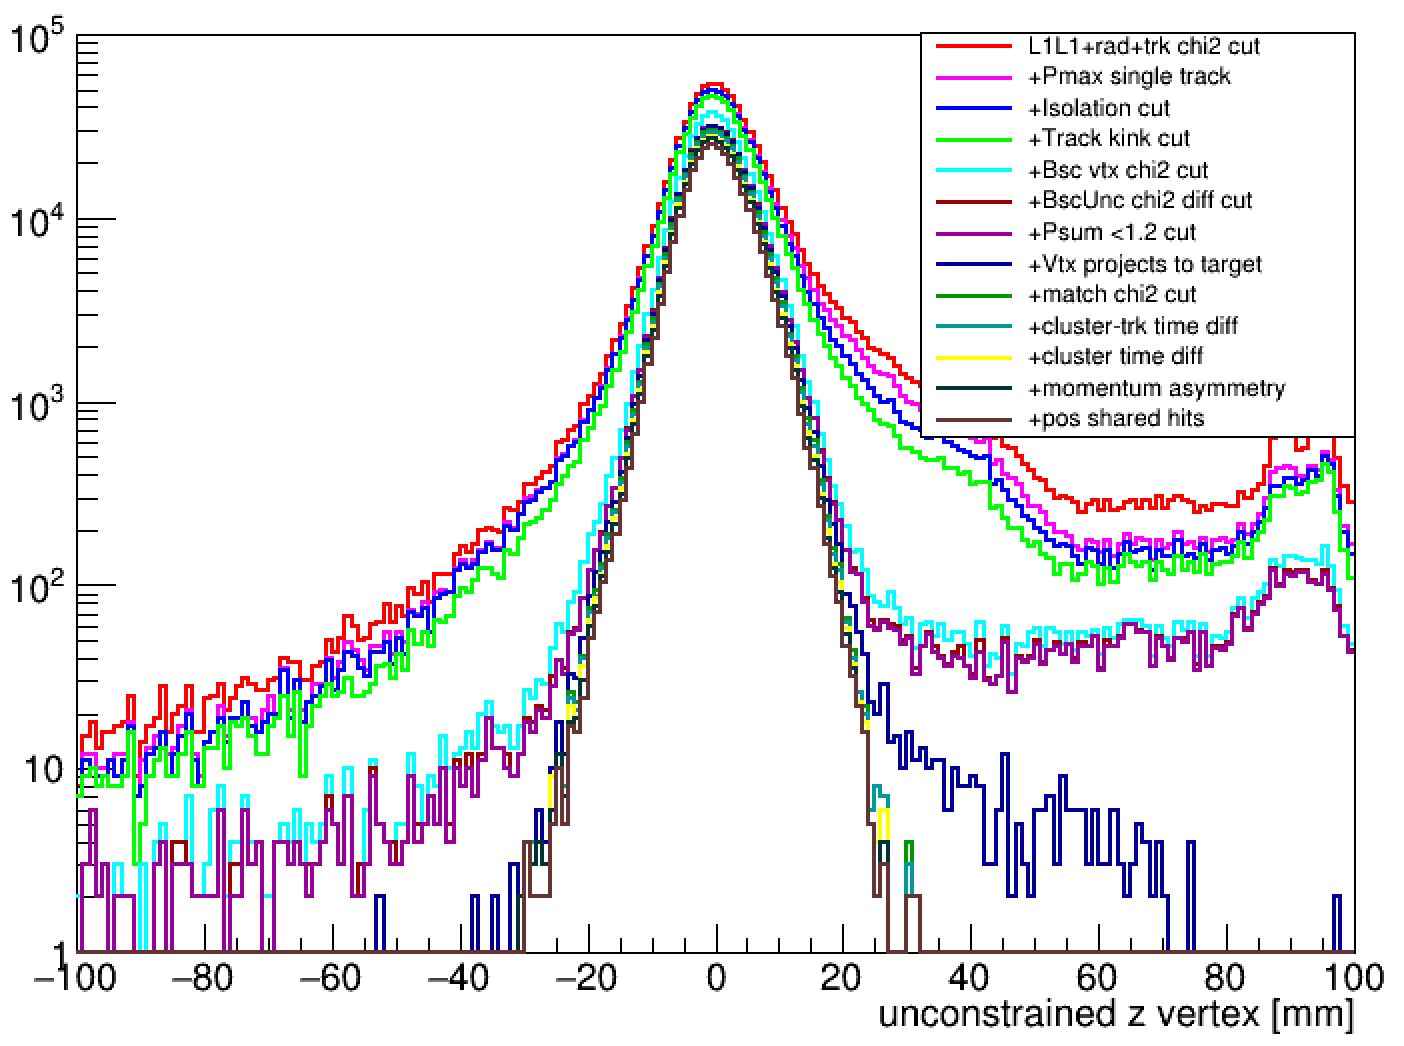
\includegraphics[width=.9\linewidth]{figs/L1L1_zvtx.png}
            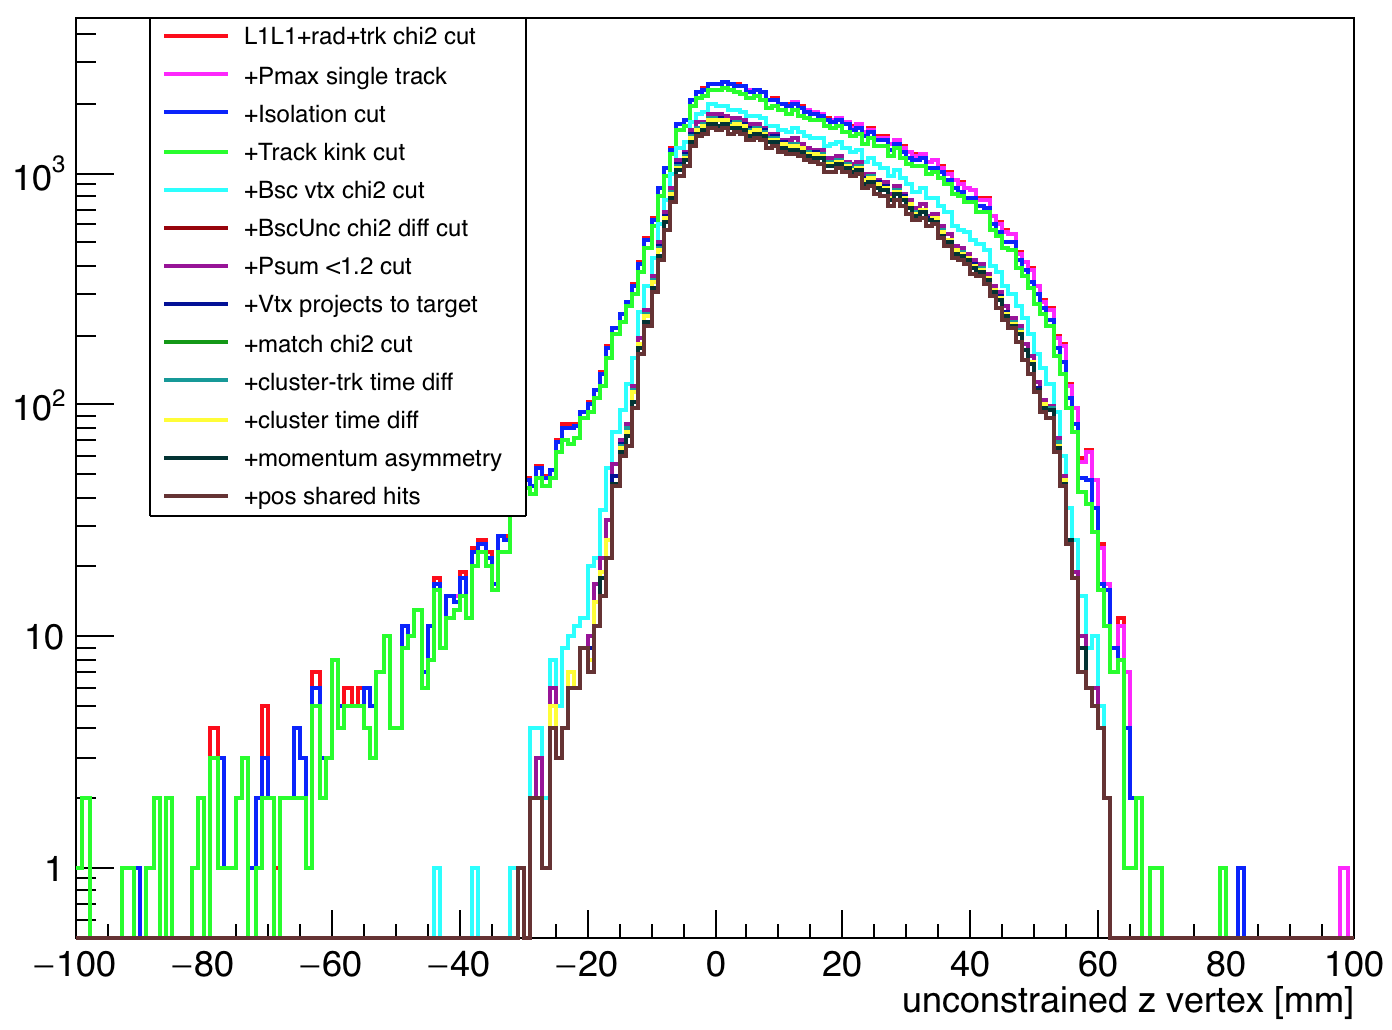
\includegraphics[width=.9\linewidth]{figs/ap40mev_zvtxCuts.png}
            \caption{
                Cut effects on the $z$ vertex distribution for data (top) a simulated 40 MeV $A^{\prime}$ for all possible couplings (bottom).}
            \label{fig:cutflow}
        \end{figure}

        \begin{figure}[th]
            \centering
            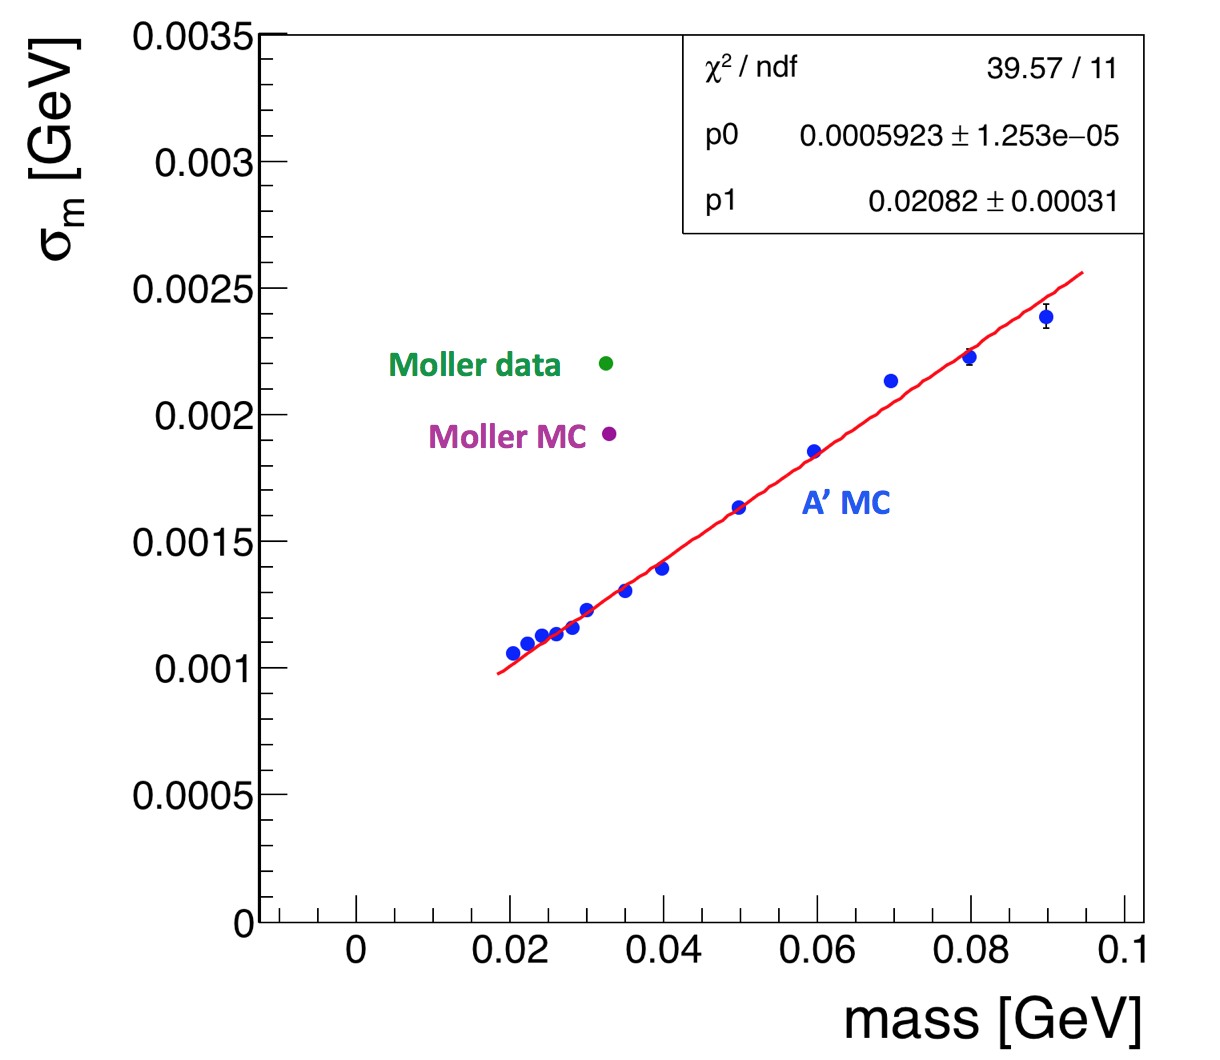
\includegraphics[width=.9\linewidth]{figs/massResolution.png}
            \caption{
                The mass resolution for M\o ller data (green), M\o ller Monte Carlo (magenta), and $A^{\prime}$ Monte Carlo (blue) is shown. The red line $\sigma_m = 0.02082m+0.0006\textrm{ GeV}$ is fit to the $A^{\prime}$ mass resolution. The difference between the Monte Carlo and data M\o ller mass resolutions is approximately 17$\%$. This scaling should be applied to the linear fit of the $A^{\prime}$ mass resolution from Monte Carlo in order to account for the difference in resolution.}
            \label{fig:massres}
        \end{figure}

    \section{Vertex Search}\label{sec:vertex}
       
        The heavy photon production rate (cross section), for both prompt and displaced vertices, is proportional to the radiative trident cross section. In looking for heavy photons with displaced vertices, the vertex distribution is examined as a function of the reconstructed invariant mass of the $e^+e^-$ pair, and events of interest are identified as originating far beyond the tails of the prompt trident backgrounds. 

We must select a downstream region when searching for a displaced heavy photon having little background. Therefore, we choose a $zCut$ which is a downstream $z$ vertex position beyond which there should be fewer than 0.5~background events per mass bin. The $zCut$ varies as a function of mass and, ideally, can be selected to minimize backgrounds whilst maximizing $A^{\prime}$ reach efficiency. Based on Poisson statistics alone, the 90$\%$ confidence limit for zero background requires us to have an expected number of $A^{\prime}$ events greater than 2.3.\\

        \begin{figure}[th]
            \centering
            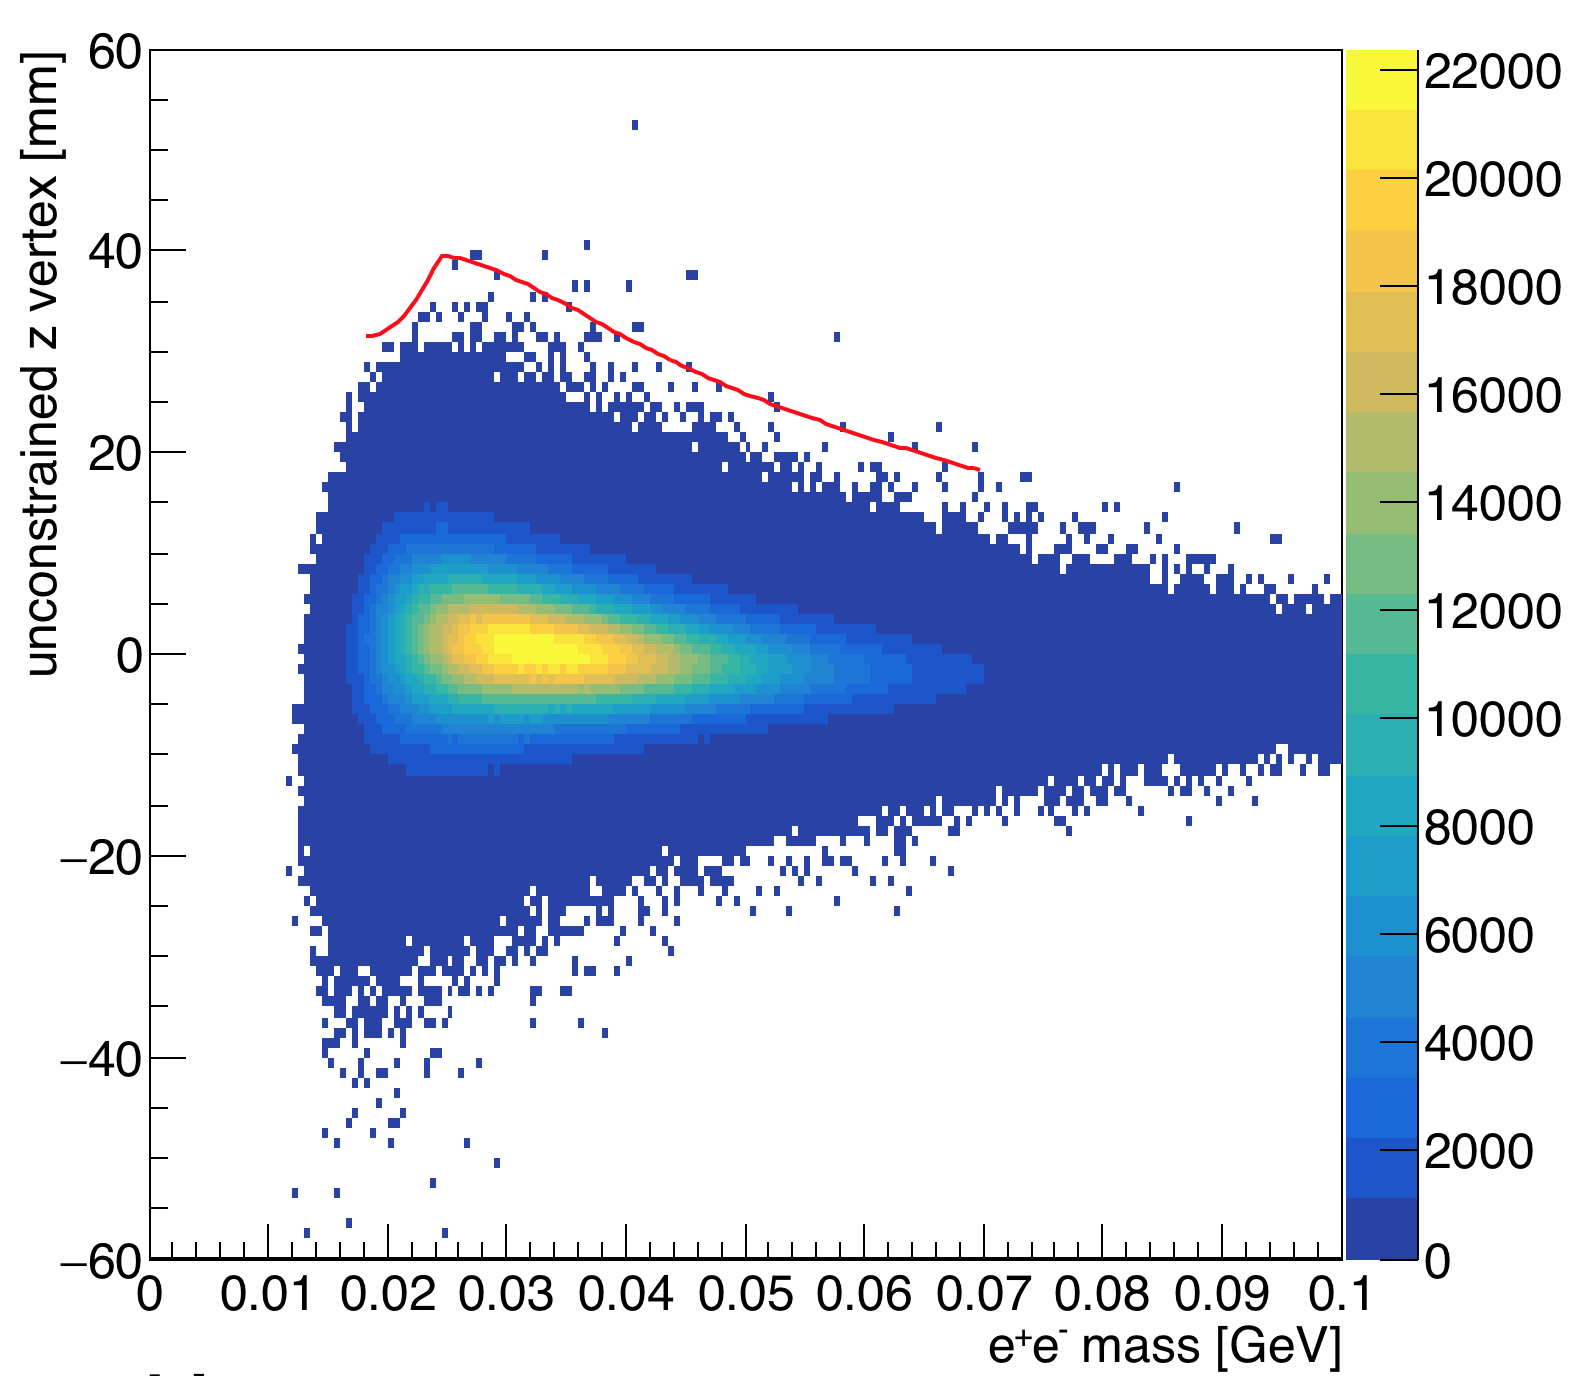
\includegraphics[width=.9\linewidth]{figs/zVm_pass8.png}
            \caption{
                The reconstructed $z$ vertex is shown versus the reconstructed mass of the $e^+e^-$ pair for all events in the 2015 L1L1 data set. The $zCut$ is obtained by slicing this distribution by mass hypothesis (window size of $\pm1.9\sigma_{m}$) and fitting each $z$ vertex distribution with Eq.~\eqref{eq:vtxFit}. The $zCut$ shown in red is the point beyond which we would expect 0.5 background events based on the fit to the tail.}
            \label{fig:zvtx}
        \end{figure}

        \begin{figure}[th]
            \centering
            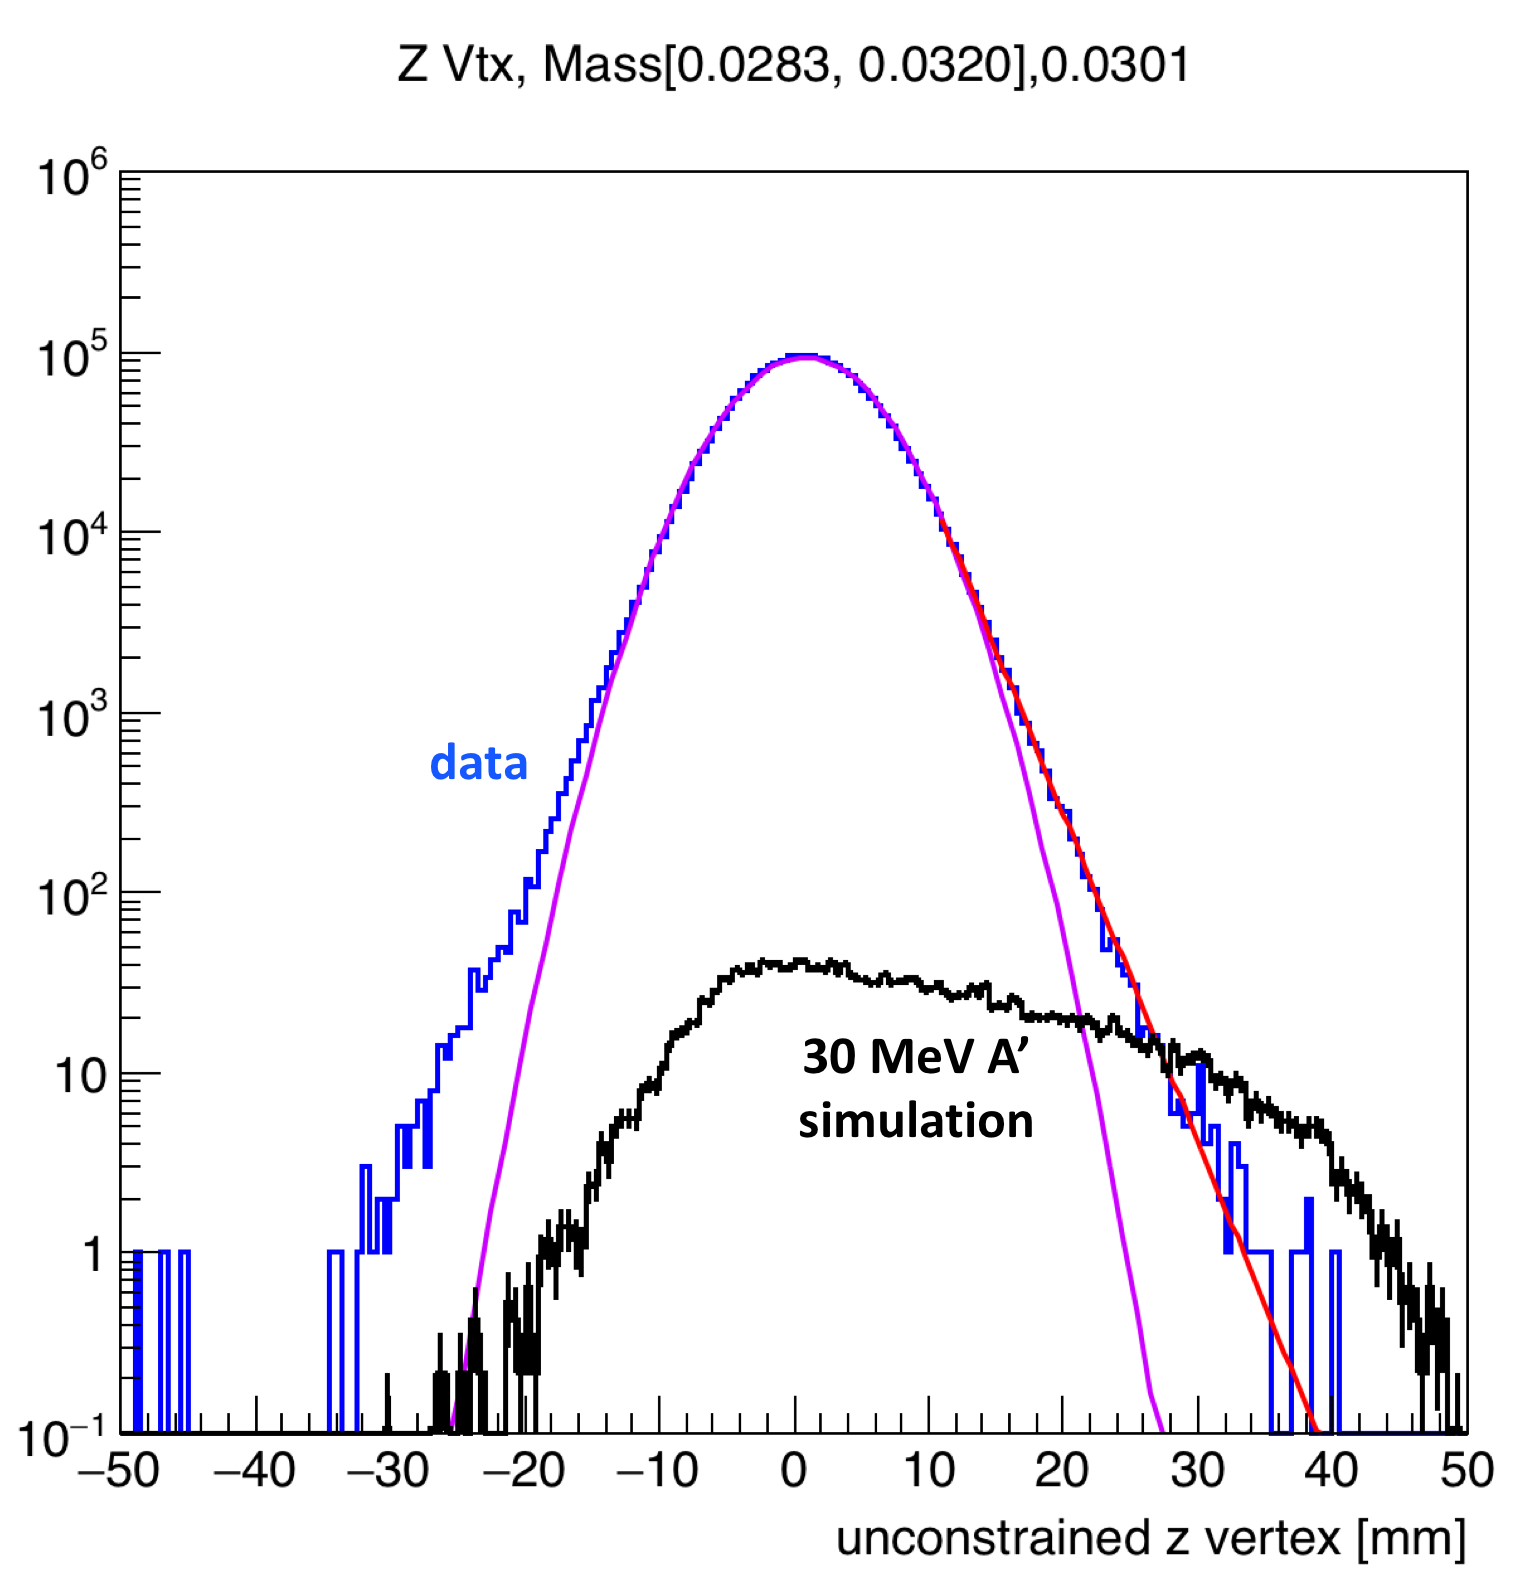
\includegraphics[width=.9\linewidth]{figs/aprimeTailPlot.png}
            \caption{
                The vertex distribution for a mass slice from data (blue) with all cuts applied and with Gaussian core fit (magenta) and downstream exponential tail fit (red) overlaid with an simulated $A^{\prime}$ Monte Carlo at the same mass (black). The tail distribution of the $A^{\prime}$ falls off more slowly compared to the distribution of events and scattering tails from the target but falls off rapidly beyond 40~mm downstream due to acceptance effects of requiring hits in Layer 1. For this particular mass slice, the $zCut$ was found to be at 37.6~mm.}
            \label{fig:aprimedistribution}
        \end{figure}
    
    \section{Vertex Results}\label{sec:vertexresults}
    
        An upper limit on the heavy photon production at a given $m_{A'}$ and $\epsilon^2$ is the maximum rate at which heavy photons could be produced, and still be consistent with the data. The confidence level used for this analysis is 90\%: in other words, if a heavy photon signal does exist at a given rate, the limit set by this analysis will (incorrectly) exclude that signal rate only 10\% of the time. The meaningful target for this analysis is the heavy photon production rate given by Equation~\eqref{eq:signal}. If the upper limit at a given $m_{A'}$ and $\epsilon^2$ is below that rate, the analysis has (at 90\% CL) excluded the possibility of a heavy photon at that $m_{A'}$ and $\epsilon^2$. Upper limits do not distinguish between a lack of sensitivity (insufficient data to say anything meaningful about the presence or absence of a signal) and the presence of a signal: the upper limit will be high in either case.

The method chosen for setting limits is the ``optimum interval'' method by Yellin \cite{ref:yellin_finding_2002}.
This method was developed for dark matter direct detection experiments, and is intended for experiments where the signal shape is known, but the backgrounds are not fully understood and there is the possibility of an unexpected background. A particular strength of the method is that it minimizes the influence of a background that is concentrated in one part of the data distribution. 

The optimum interval method sets a one-sided upper limit (with confidence level $C$) on the number of signal events $\mu$ in a one-dimensional data set, where the shape of the signal distribution is known.
For HPS, the data set is the distribution of vertex $z$ locations, after applying the mass and $z_{cut}$ cuts; the signal distribution is the $s(z)$ reported in Figure ~\ref{fig:aprimedistribution} for the $m_{A'}$ and $\epsilon^2$ being tested.

The method works by testing a proposed signal rate $\mu$ against the data with a confidence level $C$.
The cumulative distribution function of the signal, $S(z)$, is known. A change of variables is made from the measured variable $z$ to a new variable $x=\mu S(z)$. Under the signal assumption, the expected distribution of the data is uniform in $x$ with unit density, and has total width $\mu$. An interval $(x_1,x_2)$, with $x_1, x_2 \in [0,\mu]$, contains a number of expected signal events equal to its width $\Delta x = x_2-x_1$. If an unexpected background is present and is distributed differently from the signal, the data will not be distributed uniformly in $x$, and events will be spaced more widely where the background is not present.

The next step is to search for the ``optimum interval,'' the interval that most strongly rejects the proposed signal rate. This is the interval $(x_1,x_2)$ that contains the smallest number of actual events $n$ relative to its width $\Delta x$. Put another way, if the function $C_n(\Delta x,\mu)$ is the probability that all intervals of width $\Delta x$ contain more than $n$ events, the optimum interval is the $(x_1,x_2)$ that maximizes $C_n(\Delta x,\mu)$.

For the optimum interval, $x_1$ and $x_2$ always coincide with 0, $\mu$, or events in the data (otherwise the interval can be widened to increase $\Delta x$ without changing $n$). Thus the program only needs to loop over every interval between two events, of width $x$ expected events and containing $n$ actual events. The value of $C_n(\Delta x,\mu)$ for the optimum interval is called $C_{Max}$, and if it exceeds a threshold $\bar{C}_{Max}(C,\mu)$, $\mu$ is rejected with confidence level $C$.
The upper limit on $\mu$ is the value for which $C_{Max}=\bar{C}_{Max}(C,\mu)$.

The function $C_n(x,\mu)$ is the probability that all intervals containing $n$ events are narrower than this one (that is, that no interval with $n$ events has this low a ratio of actual to expected events).
The interval with largest value of $C_n(x,\mu)$ is the ``optimum interval'' that most strongly rejects the proposed signal rate.
The upper limit on $\mu$ is the value for which $C_{Max}=\bar{C}_{Max}(C,\mu)$.

The functions $C_n(x,\mu)$ and $\bar{C}_{Max}(C,\mu)$ pay the statistical penalties for using the data to pick the best interval.
Since they are not specific to the signal distribution, they are calculated using Monte Carlo and stored in lookup tables that are distributed with the software.

Here we use the optimum interval method to set a limit as we do not precisely know the shape of our background model. The optimum interval method can be used with a known background; in this case, the known background density is added to the signal density. Since the expected background for HPS falls off rapidly, relatively little is to be gained from this: after the cut in $z$, the remaining known background is tightly clustered at the edge of the range of $z$, so the optimum interval method effectively ignores it even without subtraction.
Therefore the known background is not used as an input to the optimum interval calculation.The maximum number of detectable $A^{\prime}$s and the corresponding limit as determined by the optimum interval method is shown in Fig.~\ref{fig:limit}.

Shown right in Fig.~\ref{fig:results}, the optimum interval method gives limits at 90$\%$ confidence level on $\mu$, the number of signal events past $Zcut$ and after acceptance and efficiency effects. Dividing the limit on $\mu$ by $\mu_{exp}$, the expected number of signal events for a heavy photon, gives a limit on the dimensionless ratio of the true production rate to the expected production rate for a heavy photon. A limit on $\mu / \mu_{exp}$ less than 1 means that the limit on $\mu$ is less than $\mu_{exp}$; in other words, the heavy photon is excluded (at 90$\%$ CL) at that mass and coupling. As shown in Fig.~\ref{fig:results}, we do not have sufficient data to exclude $A^{\prime}$ production at the 90$\%$ CL. 



        \begin{figure}[th]
            \centering
            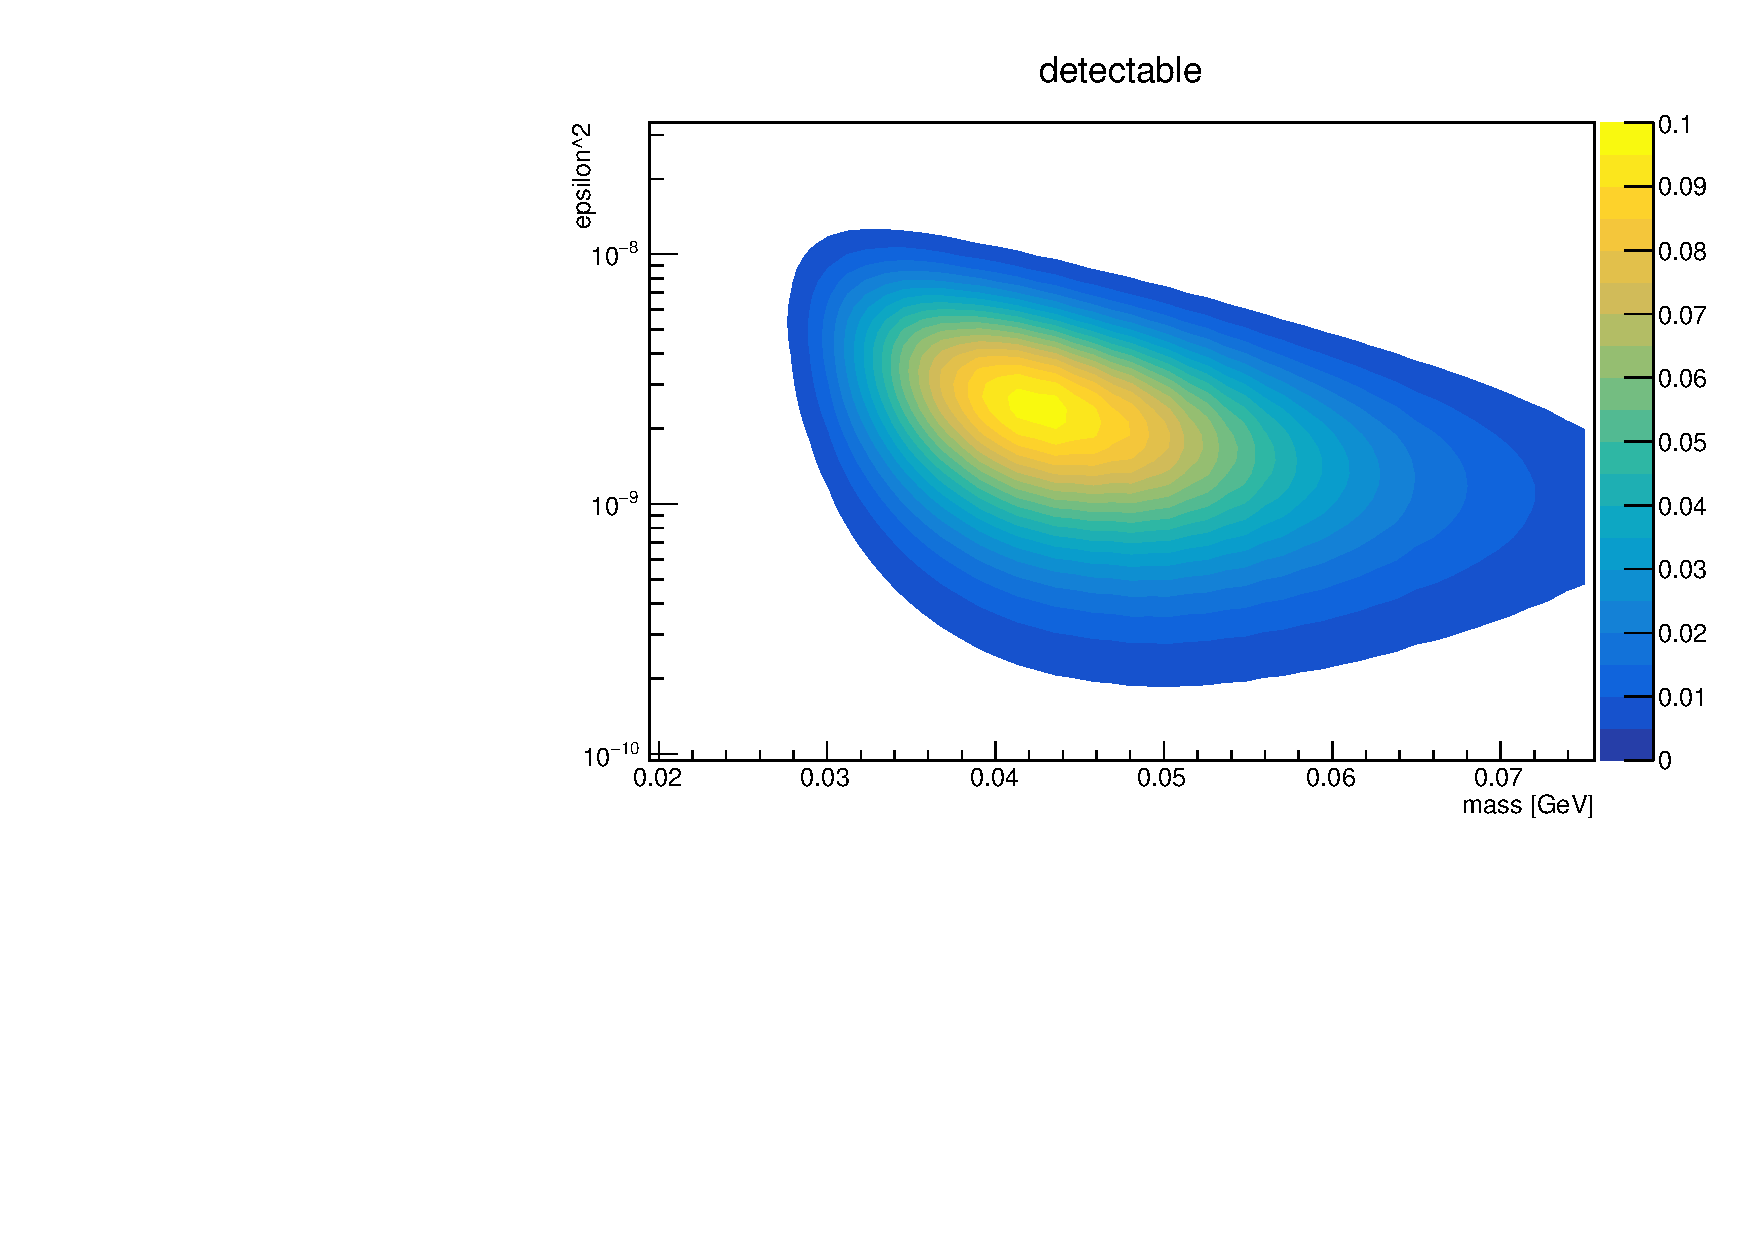
\includegraphics[width=.9\linewidth]{figs/detectable.pdf}
            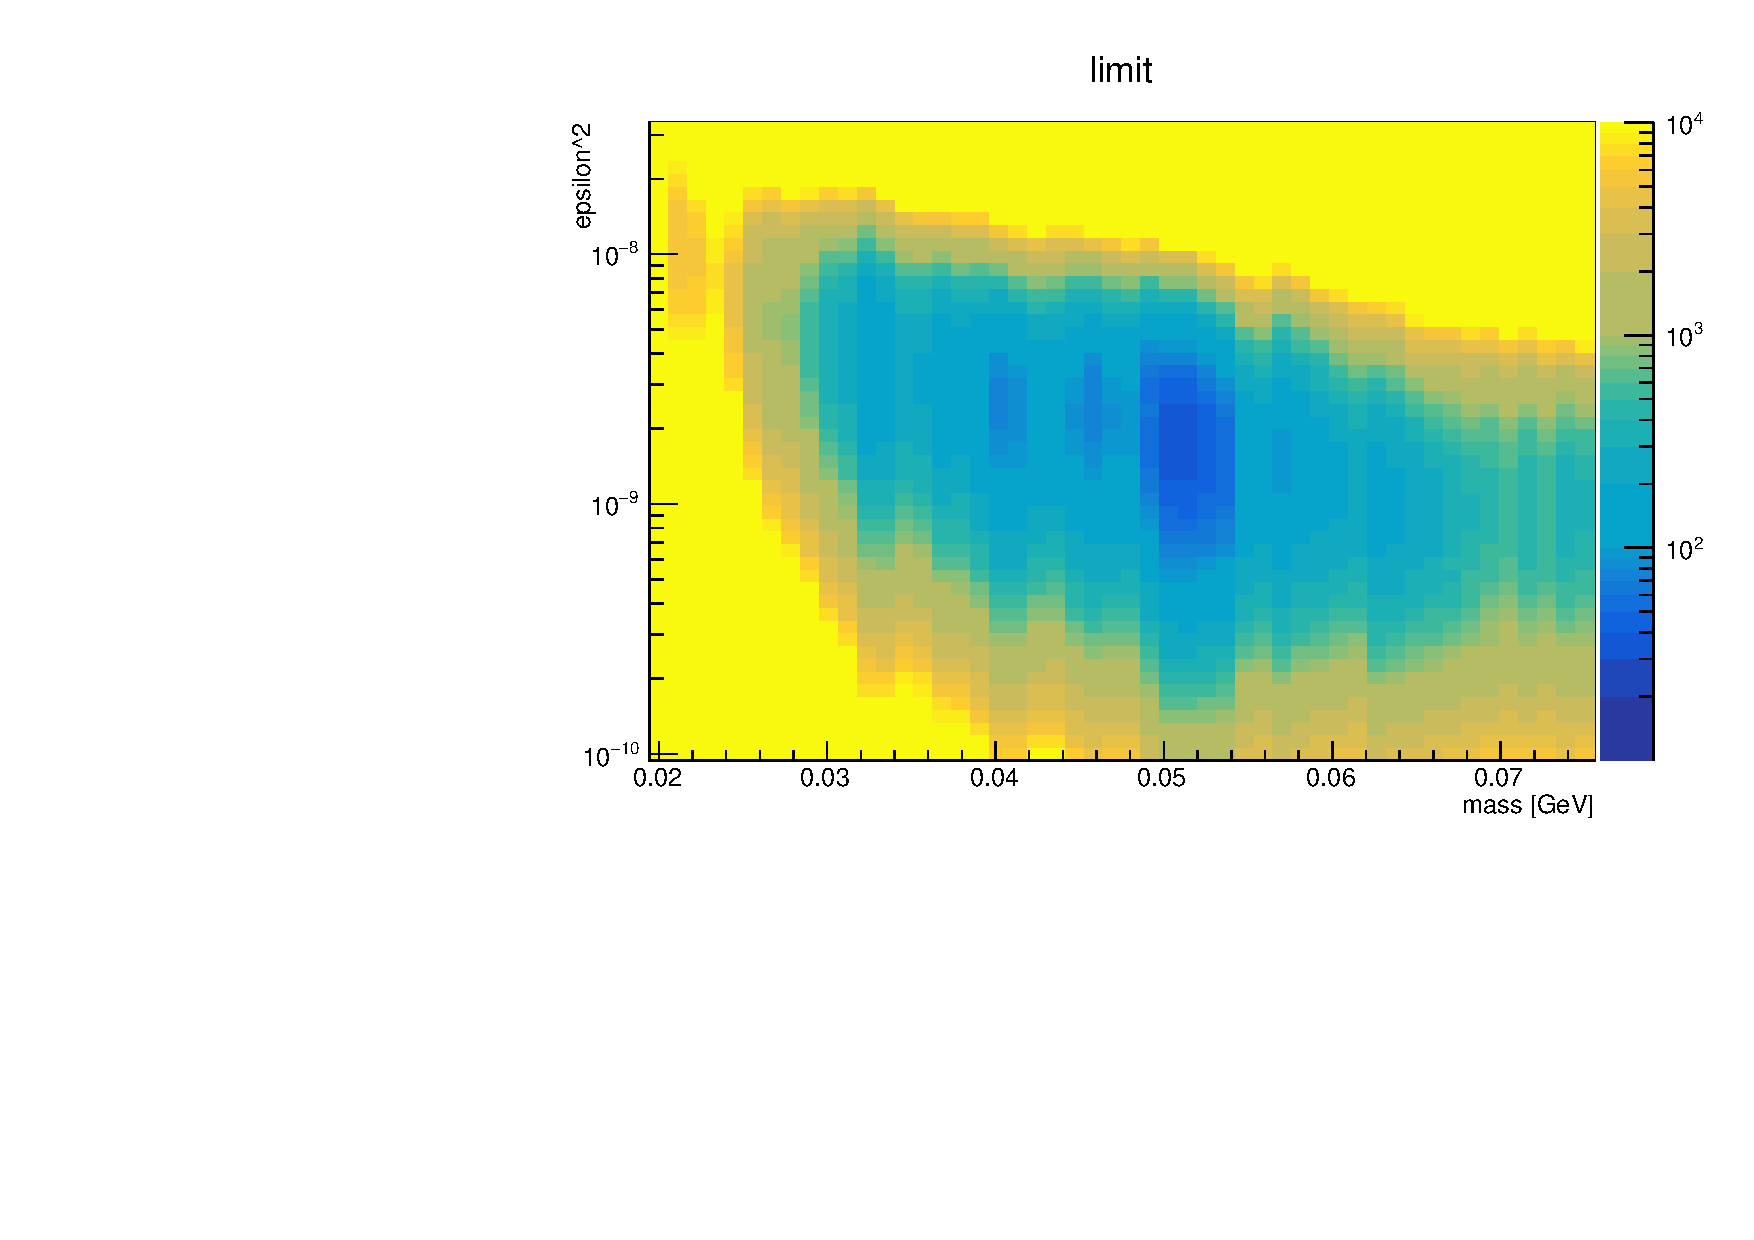
\includegraphics[width=.9\linewidth]{figs/limit.pdf}
            \caption{
                Top: The number of detectable $A^{\prime}$ events after applying all the analysis cuts and integrating over $z>Zcut$ as calculated from Equation~\eqref{eq:signal}. The number of detectable $A^{\prime}$s is found to be a maximum of $0.097$ events where $A^{\prime}$ production is maximal at a mass of 43.6 MeV and $\epsilon^2$ coupling of $2.4E-9$. Bottom: 90\% CL upper limit on $\mu/\mu_{exp}$, the ratio of the true production rate to the expected production rate for a heavy photon. A value of 1 would mean exclusion; the lowest contour on this plot is 35.7 at a mass of 51.4~MeV and coupling of $1.7E-9$. The vertical ridges in this plot correspond to the locations of events in mass space.}
            \label{fig:results}
        \end{figure}


	\section{Conclusion} \label{sec:conclusions}
        	
	Both a resonance search and a displaced vertex search for a heavy photon with a mass between 19 and 81 MeV
        which decays to an $\epem$ pair was performed.  A search for a resonance in
        the $\epem$ invariant mass spectrum yielded no significant excess and 
        established upper limits on the square of the coupling at the level of
        $6\times10^{-6}$, confirming results of earlier searches. A search for displaced vertices has been established, although no heavy photon parameter space could be excluded. While not
        covering new territory in both searches in this short engineering run, these searched did
        establish that HPS operates as designed and will, with future running,
        extend coverage for $\epsilon^2$ below the level of 10$^{-6}$ in the resonanace search and provide coverage
        of unexplored parameter space at smaller values of the coupling from a search for events with displaced vertices.

        \begin{figure}[th]
            \centering
            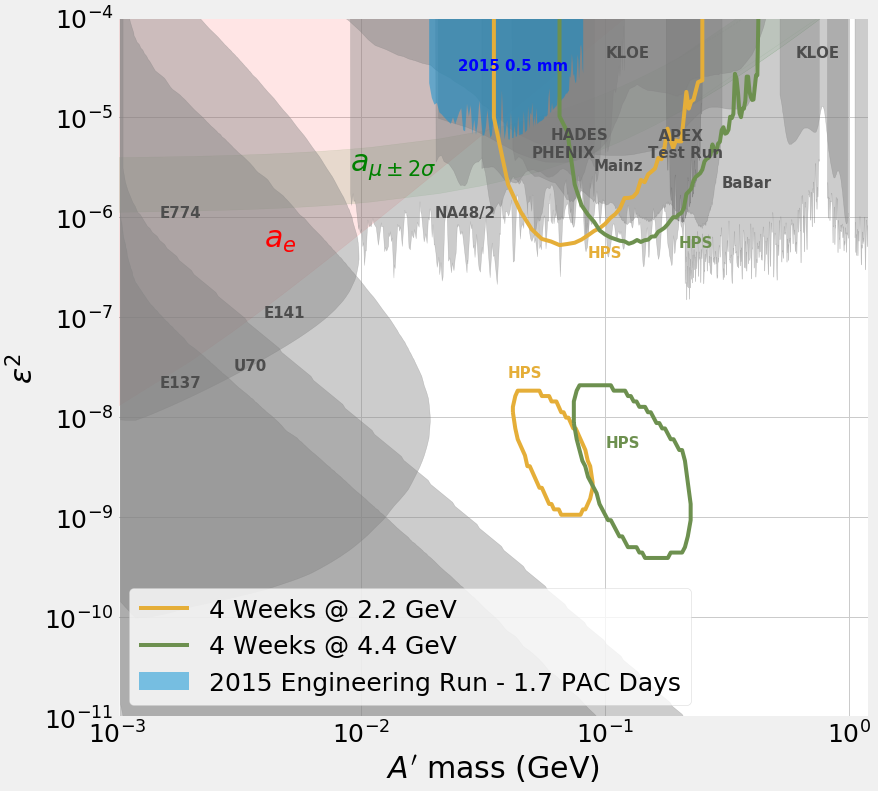
\includegraphics[width=.9\linewidth]{figs/reach_upgrade.png}
            \caption{
                Projected reach at 4 weeks of continuous beam for future running with both Layer 0 tracking upgrade and positron trigger upgrade. These upgrades recover our projected reach from the HPS proposal.}
            \label{fig:reach}
        \end{figure}

    \section{Acknowledgments}
 
        The authors are grateful for the outstanding efforts of the Jefferson 
        Laboratory Accelerator Division and the Hall B engineering group in 
        support of HPS. The research reported here is supported by the U.S.
        Department of Energy Office of Science, Office of Nuclear Physics, 
        Office of High Energy Physics, the French Centre National de la 
        Recherche Scientifique, 
        United Kingdom's Science and Technology Facilities Council (STFC),
        the Sesame project HPS@JLab funded by the French region Ile-de-France 
        and the Italian Istituto Nazionale di Fisica Nucleare. Jefferson Science
        Associates, LLC, operates the Thomas Jefferson National Accelerator
        Facility for the United States Department of Energy under Contract
        No. DE-AC05-060R23177. 
    
    \bibliography{bibliography}

\end{document}
